The following plot (figure \ref{fig plot matrix both}) is a comparison of the base values taken as a reference for the  test battery concerning the matrix multiplication on a vanilla Java code.

On the graph is plotted the base values used to compute the speedup and a measure based on the average of 5 executions. This plot demonstrates that no edge cases happened while taking the base values. The two plots show a similar behavior and even sometimes the same values.

It is worth noting that the second measure took place 2 weeks after the first one.

\begin{figure}[h!]
\centering
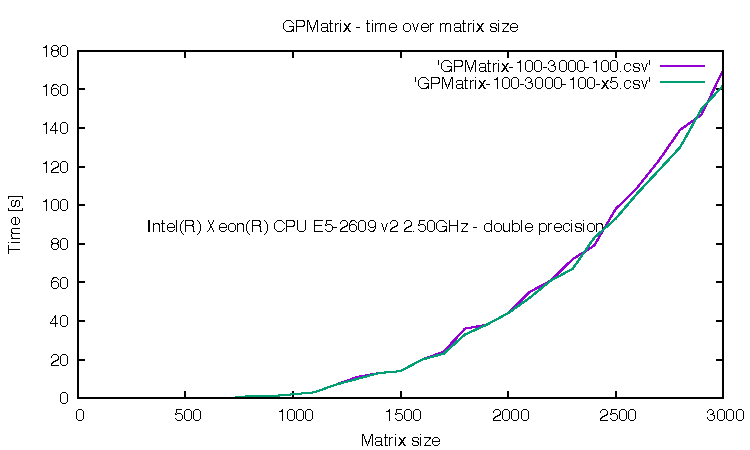
\includegraphics[width=1\textwidth]{vanilla_matrix_both.pdf}
\caption{Comparison of the base value with a measure performing an average on 5 executions.}
\label{fig plot matrix both}
\end{figure}